\documentclass{beamer}
\usetheme{Warsaw}

\usepackage[utf8]{inputenc}
\usepackage{fancybox}
\usepackage{multimedia} 
\usepackage{subfig}
\usepackage{amsmath}
\usepackage{hyperref}
\usepackage[all]{xy}
\begin{document}


\title[Angewandte Mathematik] % (optional, only for long titles)
{Angewandte Mathematik
\\

\includegraphics[scale=0.15]{images/cover}
}
\subtitle{}
\author[Dr. Johannes Riesterer] % (optional, for multiple authors)
{Dr.  rer. nat. Johannes Riesterer}

\date[KPT 2004] % (optional)
{}

\subject{Angewandte Mathematik}

\frame{\titlepage}




\begin{frame}
    \frametitle{Angewandte Mathematik}
\framesubtitle{Normen}


 \begin{block}{Normen}
\begin{align*}
 & ||x||_1 :=|x_1| + |x_2| + \cdots + |x_n| \\
 & ||x||_2 :=  \sqrt{x_1^2 + x_2^2 \cdots + x_n^2} \\
& ||x||_\infty := max_{i} |x_i|
\end{align*}
\end{block}


 \end{frame}



\begin{frame}
    \frametitle{Angewandte Mathematik}
\framesubtitle{Normen}

\begin{figure}[H]
      \centering
    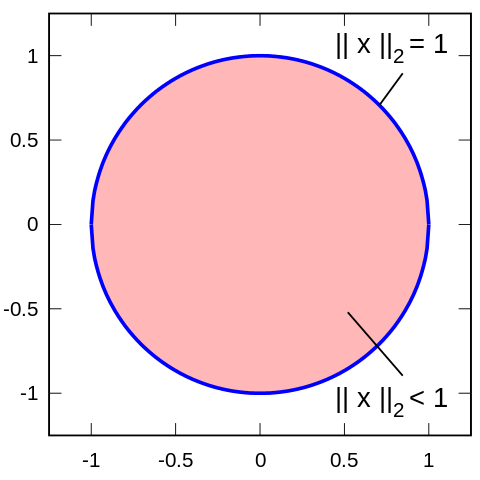
\includegraphics[width=0.4\textwidth]{images/Unit_disc_2}
\end{figure}
 \end{frame}



\begin{frame}
    \frametitle{Angewandte Mathematik}
\framesubtitle{Normen}

\begin{figure}[H]
      \centering
    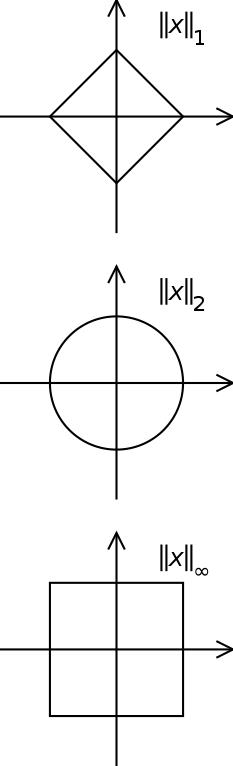
\includegraphics[width=0.2\textwidth]{images/Vector_norms}
\end{figure}

 \end{frame}



\begin{frame}
    \frametitle{Angewandte Mathematik}
\framesubtitle{Normen}

    \begin{block}{Normen}
\begin{align*}
  & x,y \in \mathbb{R}^n, \; a \in \mathbb{R} \\
& || \cdot || : \mathbb{R}^n \to \mathbb{R} \\
 & ||x|| = 0 \Leftrightarrow  x = 0 \\
& ||x+y|| \leq ||x|| + ||y|| \\
& ||a \cdot x|| = |a| \cdot ||x||
\end{align*}
\end{block}
\begin{figure}[H]
      \centering
    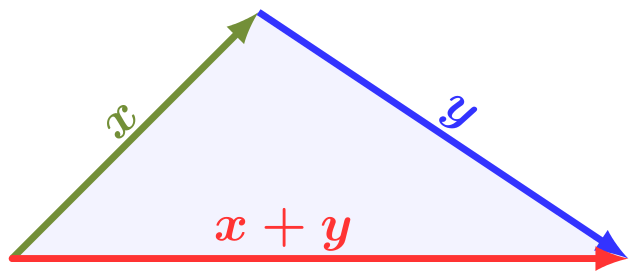
\includegraphics[width=0.6\textwidth]{images/triangle-inequality}
\end{figure}

 \end{frame}


\begin{frame}
    \frametitle{Angewandte Mathematik}
\framesubtitle{Normen}

    \begin{block}{Normen sind äquivalent}
Alle normen auf dem $\mathbb{R}^n$ lassen sich gegeneinander abschätzen.

\end{block}
    \begin{block}{Normen}
Man kann skalierte Kugeln der verschiedenen Normen ineinander schachteln....
\end{block}


 \end{frame}



\begin{frame}
    \frametitle{Angewandte Mathematik}
\framesubtitle{Skalarprodukt}
 \begin{block}{Skalarprodukt}
\begin{align*}
  & x,y,z \in \mathbb{R}^n, \; a,b \in \mathbb{R} \\
& < \cdot, \cdot > : \mathbb{R}^n \times \mathbb{R}^n  \to \mathbb{R} \\
& <x+y, z> = <x,z> + <y,z> \\
& <x, y+z> = <x,y> + <x,z> \\
& <a\cdot x, b \cdot y> = a \cdot b \cdot <x,y>  
\end{align*}
\end{block}
 \end{frame}



\begin{frame}
    \frametitle{Angewandte Mathematik}
\framesubtitle{Skalarprodukt}
 \begin{block}{Skalarprodukt}
\begin{align*}
<x,y>_2 = x_1 \cdot y_1 + x_2 \cdot y_2 + \cdots + x_n \cdot y_n 
\end{align*}
\end{block}

 \begin{block}{Skalarprodukt}
\begin{align*}
||x||_2 = \sqrt{<x,x>_2} 
\end{align*}
\end{block}

 \end{frame}


\begin{frame}
    \frametitle{Angewandte Mathematik}
\framesubtitle{Fehleranalyse}
    \begin{block}{Skalarprodukt}
\begin{align*}
<x,y> = \frac{\cos(\varphi)}{||x|| \cdot ||y||}
\end{align*}
\end{block}
\begin{figure}[H]
      \centering
    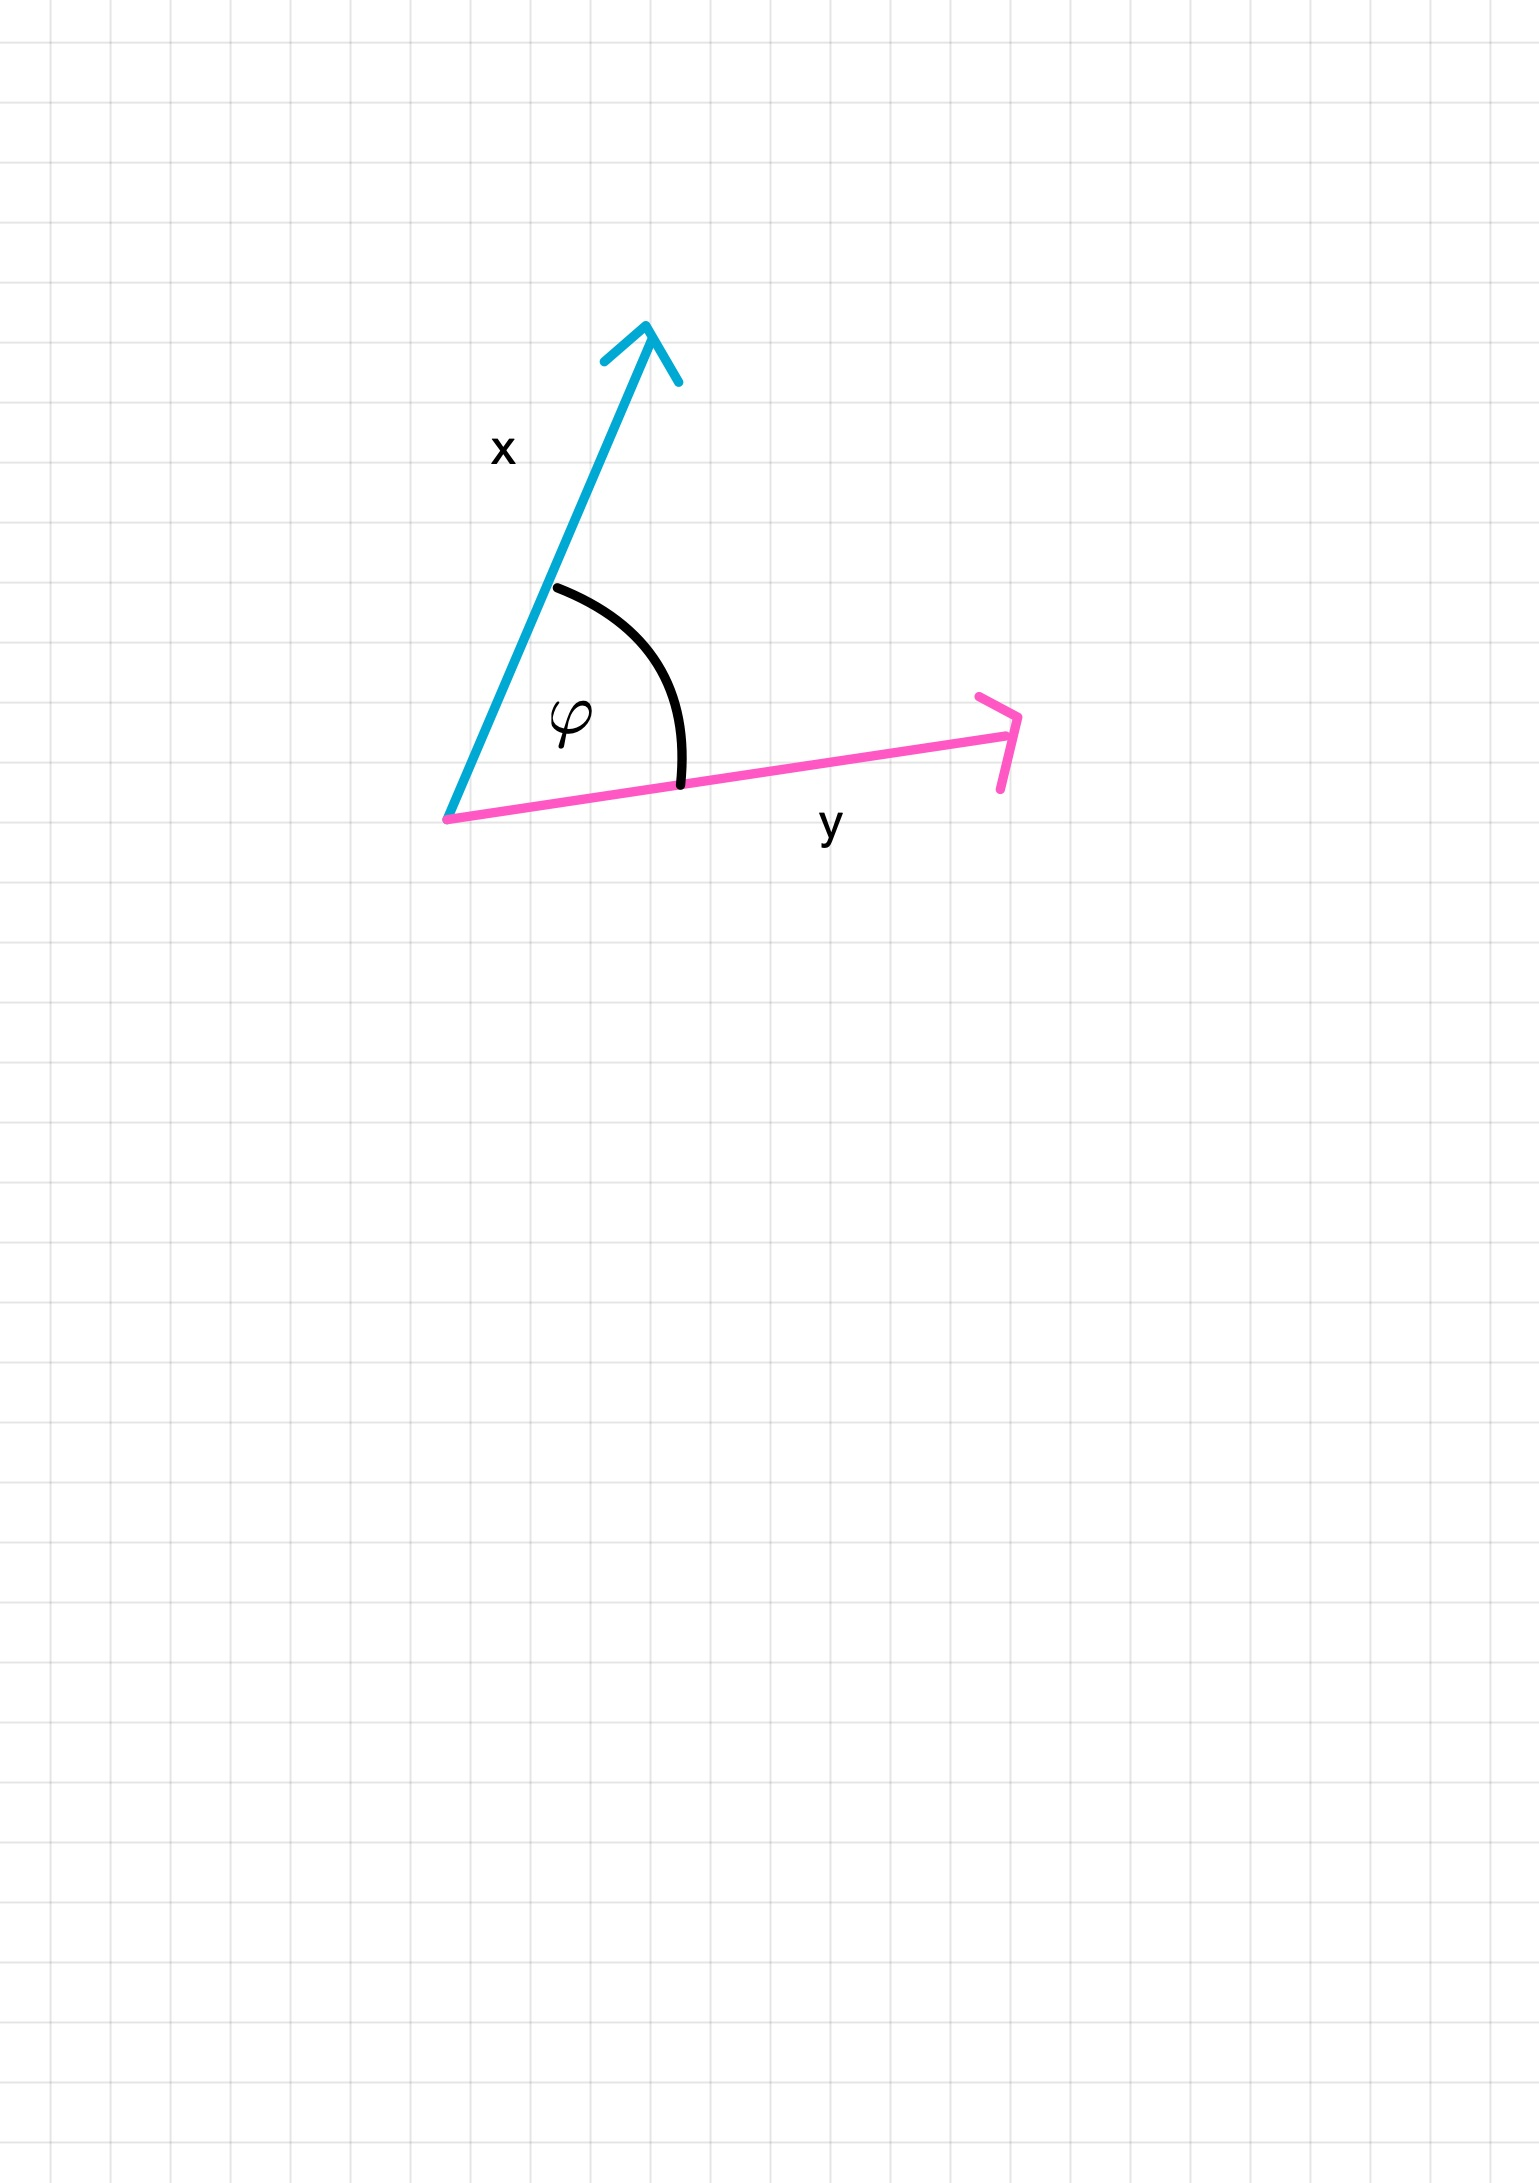
\includegraphics[width=0.6\textwidth]{images/angle}
\end{figure}
 \end{frame}





\begin{frame}
    \frametitle{Angewandte Mathematik}
\framesubtitle{Normen}
 \begin{block}{Abstand}
\begin{align*}
d(x,y) := ||x-y||
\end{align*}
\end{block}
 \begin{block}{Abstand}
\begin{align*}
& d(x,y)  = 0 \Leftrightarrow x = y \\
& d(x,y)  > 0 \Leftrightarrow x \neq y \\
& d(x,z)  \leq  d(x,y) + d(y,z) 
\end{align*}
\end{block}
 \end{frame}

\end{document}

